\documentclass[aspectratio=169]{beamer}

\graphicspath{{figs}}

\usepackage{iftex}
\ifPDFTeX
    \usepackage[T2A]{fontenc}
    \usepackage[utf8]{inputenc}
\else
    \usepackage{fontspec}
    \setmainfont{cmunrm.otf}[BoldFont=cmunbx.otf,ItalicFont=cmunti.otf]
    \setsansfont{cmunss.otf}[BoldFont=cmunsx.otf,ItalicFont=cmunsi.otf]
\fi
\usepackage[english,russian]{babel}
\usepackage{cmap}
\usepackage{tikz}
\usepackage{array}
\usepackage{multicol}
\usepackage{booktabs}
\usepackage{csquotes}
\usepackage{amssymb,amsfonts,amsmath}

\usecolortheme{beaver}
\usefonttheme[onlymath]{serif}
\setbeamertemplate{navigation symbols}{}
\setbeamertemplate{footline}[page number]
\setbeamertemplate{blocks}[rounded=true,shadow=true]
\setbeamersize{text margin left=0.5cm,text margin right=0.5cm}
\setbeamertemplate{frametitle}[default][center]
\setbeamercolor{frametitle}{fg=black}

\begin{document}

\begin{frame}[t]{Нарезка патентов для векторного поиска и RAG}
    \begin{alertblock}{Суть}
        \small
        Нарезка по длине смешивает в одном фрагменте разные разделы патента.
        Строим фрагменты $c_j$ по разделам $s_k$: смысл не размывается, а вклад каждого раздела в поиск можно измерить.
    \end{alertblock}

    \begin{columns}[T]
        \begin{column}{0.55\textwidth}
            \begin{block}{Термины и обозначения}
                \footnotesize
                \textbf{Патент} $d$: документ из разделов $s_k$.\\
                \textbf{Нарезка}: разбиение $d$ на фрагменты $c_j$.\\
                \textbf{Векторный поиск}: выбор $c_j$, близких к запросу по эмбеддингам.\\
                \textbf{RAG}: ответ языковой модели по найденным $c_j$.
            \end{block}

            \centering
            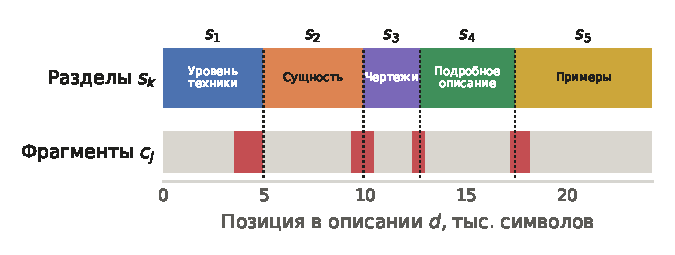
\includegraphics[width=0.9\textwidth]{sections_chunks}
        \end{column}
        \begin{column}{0.43\textwidth}
            \begin{exampleblock}{Эксперимент}
                \footnotesize
                Заголовки разделов ищутся по ключевым словам: 291 вариант заголовка сводится к 8 типам разделов.

                \smallskip
                \textbf{Результат} на 37\,727 патентах:
                \begin{itemize}
                    \item разделы выделены у \textbf{98,5\%} патентов;
                    \item обычно 5--6 разделов на патент;
                    \item уровень техники у 91\%, сущность у 86\%, подробное описание у 89\% (63\% текста);
                    \item красные фрагменты по 10 предложений пересекают границу раздела.
                \end{itemize}
            \end{exampleblock}
        \end{column}
    \end{columns}
\end{frame}

\end{document}
